%%UTF-8
\documentclass[twoside]{nputhesis}
%\documentclass[oneside]{nputhesis}

\usepackage{amsmath}
\usepackage{amsfonts}
\usepackage{booktabs}
\usepackage{multirow}
\usepackage{graphicx}

\usepackage{lipsum}

\schoolno{10699}
%\classno{}
%\secretlevel{}
%\title{\LaTeX 论文模板之模板模板模板}
\title[\LaTeX\ template]{\LaTeX 论文模板之模板模板模板}
\author[Yimu Shu]{水易木}
\authorno{2014201852}
\major[Math]{数学}
\supervisor[Shan]{山}
\applydate[September 2016]{2016~年~9~月}
\support{本文研究得到某某基金(编号:XXXXXXX)资助。}

\begin{document}
\makecover
\frontmatter
% 中文摘要
\begin{abstract}
  中文 \lipsum[2-3]
  \begin{keywords}
   中文, 摘要
  \end{keywords}
\end{abstract}
% 英文摘要
\begin{Abstract}
  \lipsum[1-4] 
  \begin{Keywords}
  English, Abstract
  \end{Keywords}
\end{Abstract}
\tableofcontents 

\mainmatter
\chapter{简介}
\section{运行环境}
\subsection{操作系统}
\begin{equation}
  a^2+b^2=c^2
\end{equation}
我是正文 我是正文 我是正文 我是正文 我是正文 我是正文 我是正文 
我是正文 我是正文 我是正文 我是正文 我是正文 我是正文 我是正文 
我是正文 我是正文 我是正文 我是正文 我是正文 我是正文 我是正文 
我是正文 我是正文 我是正文 我是正文 我是正文 我是正文 我是正文 
我是正文 我是正文 我是正文 我是正文 我是正文 我是正文 我是正文 
我是正文 我是正文 我是正文 我是正文 我是正文 我是正文 我是正文
我是正文 我是正文 我是正文 我是正文 我是正文 我是正文 我是正文
我是正文 我是正文 我是正文 我是正文 我是正文 我是正文 我是正文
我是正文 我是正文 我是正文 我是正文 我是正文 我是正文 我是正文
我是正文 我是正文 我是正文 我是正文 我是正文 我是正文 我是正文
\begin{table}
  \caption{测试表格}
  \centering
  \begin{tabular}{cccccc}
    \toprule
    & $h$ & $L^2$ error & Order & $L^{(\alpha,\beta)}$ error & Order \\
    \midrule
    \multirow{5}{4em}{$\alpha=0.85$\\ $\beta = 0.85$}
    & 1/4   & 3.8571e-04 &      - & 3.0781e-03 &      -\\
    & 1/8   & 1.3035e-04 & 1.5651 & 1.2640e-03 & 1.2840\\
    & 1/16  & 3.8665e-05 & 1.7533 & 5.2782e-04 & 1.2599\\
    & 1/48  & 4.9386e-06 & 1.8731 & 1.5519e-04 & 1.1142\\
    \bottomrule
  \end{tabular}
\end{table}
\cite{Ji2015}\cite{Grisvard2011}\cite{Roop2006}
\cite{Roop2004}\cite{Gorenflo2001}\cite{Oldham1974}\cite{Berthold1992}
\cite{Guo2011}
\chapter{实现}
\section{实现思路}
\begin{equation}
  E=mc^2
\end{equation}
\begin{figure}
  \centering
  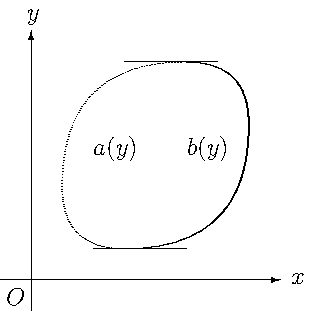
\includegraphics{figures/fig1-1.pdf}
  \hskip 10pt
  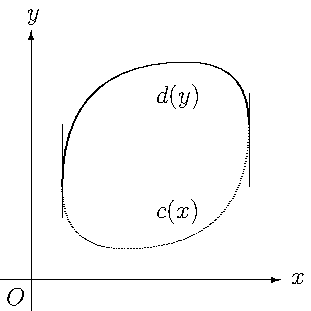
\includegraphics{figures/fig1-2.pdf}
  \caption{测试图-区域}
\end{figure}
\begin{figure}
  \centering
  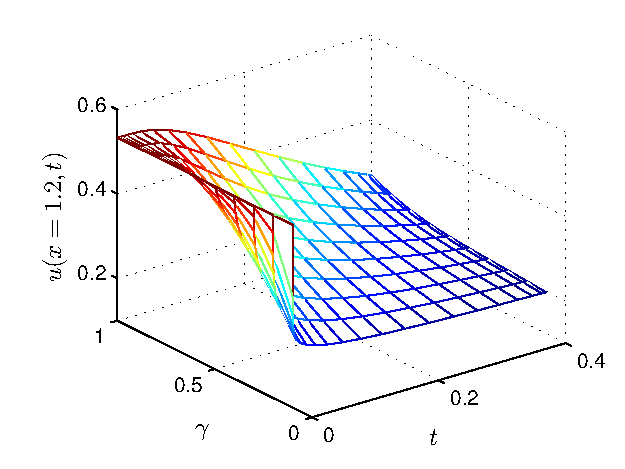
\includegraphics{figures/fig2.pdf}
  \caption{测试图-三维图}
\end{figure}
%\begin{figure}
  %\centering
  %\includegraphics{figures/fig3.eps}
  %\caption{测试图-三维图}
%\end{figure}
%\begin{figure}
  %\centering
  %\includegraphics[width=0.3\textwidth]{figures/nwpu.jpg}
  %\caption{测试图-工大图标}
%\end{figure}
\lipsum[4-8]
\section{实现代码}
\lipsum[2-4]

\backmatter
\bibliographystyle{nputhesis}
\bibliography{Reference}

\Appendix
This is appendix.

\Thanks
This is a thanks.

\Work
% TODO 如何直接引用使参考文献的内容显示在这里

\statement
\end{document}

